\documentclass[10pt]{article}
\usepackage[margin=0.9in]{geometry}
\usepackage{amsmath,graphicx,booktabs,tikz,float}
\usepackage[font=small,labelfont=bf]{caption}
\usetikzlibrary{arrows.meta,positioning,calc}
\tikzset{>=Stealth, blk/.style={draw, minimum height=7mm, minimum width=12mm, align=center, font=\small}}

\title{Adaptive TX FFE with Sign-Sign LMS:\\a Symbol-Rate Simulation on a Backplane Channel}
\author{}
\date{}

\begin{document}
\maketitle
\vspace{-1.5em}

\section*{Goal}
Reproduce the dual-loop TX FFE adaptation of Stojanovi\'c et al.\ (JSSC 2005)
in simulation: a 4-tap transmit FFE adapted by sign-sign LMS from a single
receiver-side error sampler, over a real backplane channel (ECEN720 T20 server
thru, 10\,Gb/s NRZ). The unequalized channel loses 27.6\,dB at Nyquist and its
worst-case (peak-distortion) eye is closed.

\section*{System}
\begin{figure}[h]
\centering
\begin{minipage}[c]{0.36\linewidth}
  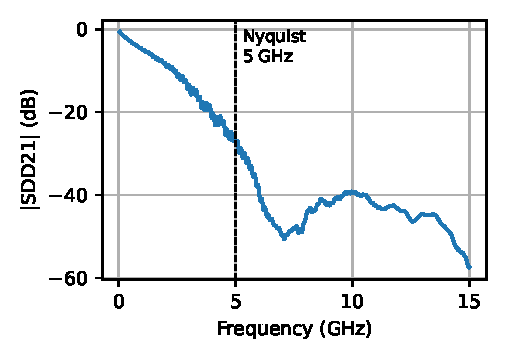
\includegraphics[width=\linewidth]{figures/s21.pdf}
\end{minipage}\hfill
\begin{minipage}[c]{0.6\linewidth}
\centering
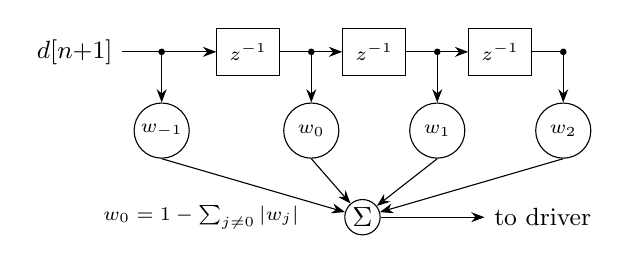
\begin{tikzpicture}[x=1cm, y=1cm]
  % delay line
  \node[font=\small, left] (din) at (0,0) {$d[n{+}1]$};
  \foreach \i/\x in {1/1.6, 2/3.2, 3/4.8} \node[blk, minimum width=8mm, minimum height=6mm] (z\i) at (\x,0) {\scriptsize $z^{-1}$};
  \draw[->] (0,0) -- (z1.west);
  \draw[->] (z1.east) -- (z2.west);
  \draw[->] (z2.east) -- (z3.west);
  % taps
  \foreach \i/\x/\w in {0/0.5/{-1}, 1/2.4/0, 2/4.0/1, 3/5.6/2} {
    \fill (\x,0) circle (1.2pt);
    \node[draw, circle, inner sep=0.5pt, minimum size=7mm, font=\scriptsize] (w\i) at (\x,-1.0) {$w_{\w}$};
    \draw[->] (\x,0) -- (w\i.north);
  }
  \draw (z3.east) -- (5.6,0);
  % sum
  \node[draw, circle, inner sep=1pt] (sum) at (3.05,-2.1) {$\Sigma$};
  \foreach \i in {0,1,2,3} \draw[->] (w\i.south) -- (sum);
  \draw[->] (sum.east) -- (4.6,-2.1) node[right, font=\small] {to driver};
  \node[font=\scriptsize, align=left] at (1.0,-2.1) {$w_0 = 1-\sum_{j\neq0}|w_j|$};
\end{tikzpicture}
\end{minipage}
\caption{Left: channel loss. Right: symbol-spaced TX FFE (one pre-tap, two
post-taps). The TX peak swing is fixed, so the main tap takes whatever the
other taps leave: $\sum_j |w_j| = 1$.}
\end{figure}

\begin{figure}[h]
\centering
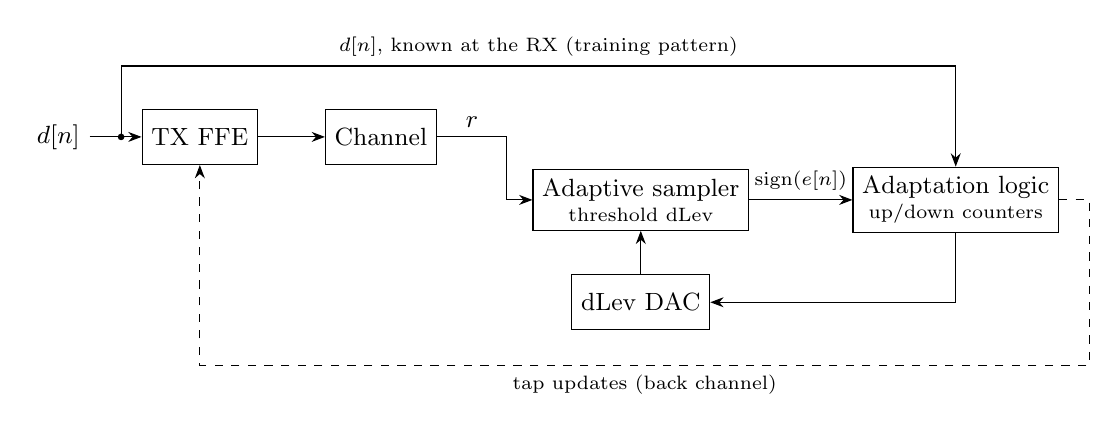
\begin{tikzpicture}[x=1cm, y=1cm]
  \node[blk] (ffe) at (0,0) {TX FFE};
  \node[blk] (ch) at (2.3,0) {Channel};
  \node[blk] (err) at (5.6,-0.8) {Adaptive sampler\\[-2pt]\scriptsize threshold dLev};
  \node[blk] (eng) at (9.6,-0.8) {Adaptation logic\\[-2pt]\scriptsize up/down counters};
  \node[blk] (dac) at (5.6,-2.1) {dLev DAC};
  \draw[->] (-1.4,0) node[left, font=\small] {$d[n]$} -- (ffe);
  \fill (-1.0,0) circle (1.2pt);
  \draw[->] (-1.0,0) |- (9.6,0.9) node[pos=0.75, above, font=\scriptsize]
    {$d[n]$, known at the RX (training pattern)} -- (eng.north);
  \draw[->] (ffe) -- (ch);
  \draw[->] (ch.east) -- node[above, font=\small] {$r$} (3.9,0) |- (err.west);
  \draw[->] (err.east) -- node[above, font=\scriptsize] {$\mathrm{sign}(e[n])$} (eng.west);
  \draw[->] (eng.south) |- (dac.east);
  \draw[->] (dac.north) -- (err.south);
  \draw[->, dashed] (eng.east) -- (11.3,-0.8) |- (0,-2.9)
    node[pos=0.75, below, font=\scriptsize] {tap updates (back channel)} -- (ffe.south);
\end{tikzpicture}
\caption{Adaptation loop as simulated. One extra comparator, whose threshold
is the dLev DAC, gives $\mathrm{sign}(e)$ directly; no ADC is needed. The data
correlated against $\mathrm{sign}(e)$ is the transmitted $d[n]$, i.e.\ a known
training pattern (or error-free RX decisions).}
\end{figure}

\section*{Algorithm}
With $e[n] = \mathrm{dLev} - r[n]$, the two loops of the paper are
\begin{align*}
  w_j &\leftarrow w_j + \Delta_w\,\mathrm{sign}\Big(\textstyle\sum_n \mathrm{sign}(e[n])\, d[n-j]\Big), \quad j\neq 0,
  &
  \mathrm{dLev} &\leftarrow \mathrm{dLev} - \Delta_{\mathrm{dLev}}\,\mathrm{sign}\Big(\textstyle\sum_n \mathrm{sign}(e[n])\Big),
\end{align*}
summed over a block of symbols (one step per block, as an up/down counter would).
\begin{itemize}\itemsep0pt
  \item \textbf{One sampler.} It sits at $+\mathrm{dLev}$, so only symbols with $d[n]=+1$ contribute.
  \item \textbf{Main tap from the constraint.} Scaling all taps and dLev together leaves every
        $\mathrm{sign}(e)$ unchanged, so the two loops alone cannot fix the overall scale (and can
        drift to all-zero). Setting $w_0 = 1-\sum_{j\neq0}|w_j|$ removes that freedom. dLev cannot
        be found first: it is the equalized main cursor, which depends on the final taps.
  \item \textbf{Averaged, it is zero-forcing.} $E\big[e[n]\,d[n-j]\big]$ is the residual ISI at cursor
        $j$, so each tap drives its own cursor to zero, even when the unequalized eye is closed.
  \item \textbf{Noise helps.} Without sampler noise the residual ISI takes few discrete values and
        $\mathrm{sign}(e)$ has a dead zone around the solution (tap error $\sim$5$\times$ larger).
\end{itemize}

\section*{Simulation}
Symbol-rate model in Python: the channel is its pulse response sampled once per UI at the peak
(3 pre-, 40 post-cursors); TX FFE and channel run as a continuous stream across blocks.
3000 blocks $\times$ 512 symbols, $\Delta_w=\Delta_{\mathrm{dLev}}=10^{-3}$, 5\,mV rms sampler
noise. The loop uses the transmitted symbols, aligned to each received sample, in place of RX
decisions. Eyes are then checked with a waveform-level link (32 samples/UI, full S-parameter channel).

\section*{Results}
\begin{figure}[h]
\centering
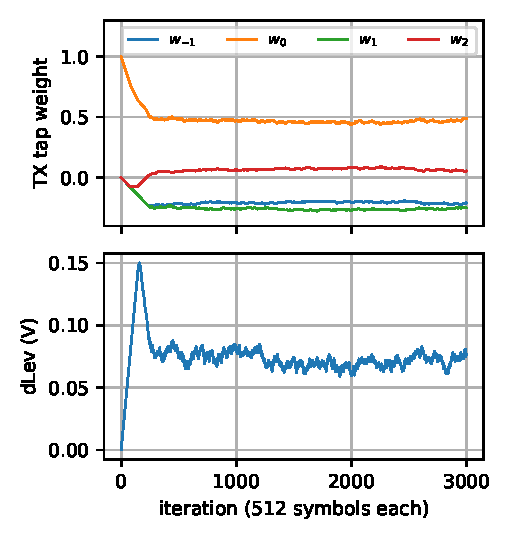
\includegraphics[width=0.42\linewidth]{figures/convergence.pdf}\hspace{4mm}
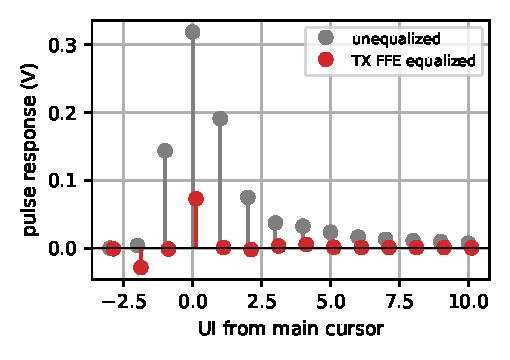
\includegraphics[width=0.42\linewidth]{figures/pulse.pdf}
\caption{Left: taps and dLev converge together in $\sim$300 blocks; dLev overshoots, then
follows the main cursor down as pre-emphasis takes swing. Right: UI-spaced pulse response;
the cursors within the FFE span ($-1$, $+1$, $+2$) are driven to zero.}
\end{figure}

\begin{figure}[h]
\centering
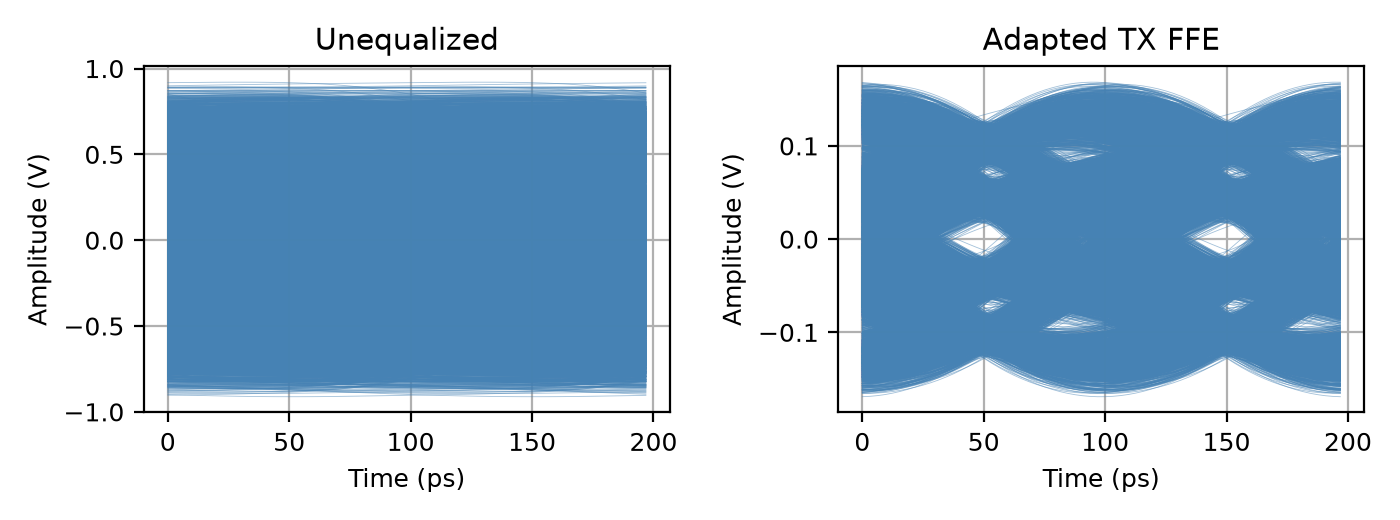
\includegraphics[width=0.78\linewidth]{figures/eyes.png}
\caption{10\,000 random bits through the waveform-level link, before and after adaptation.}
\end{figure}

\begin{table}[h]
\centering\small
\begin{tabular}{lccc}
\toprule
 & main cursor & $\sum|\text{ISI}|$ & PDA eye height \\
\midrule
Unequalized & 0.319\,V & 0.630\,V & $-0.622$\,V (closed) \\
Adapted TX FFE & 0.073\,V & 0.061\,V & $+0.024$\,V (open) \\
\bottomrule
\end{tabular}
\caption{Adapted taps $[w_{-1}, w_0, w_1, w_2] = [-0.212, 0.470, -0.256, 0.061]$
(mean of the last 500 blocks); the exact zero-forcing solution is
$[-0.205, 0.462, -0.261, 0.072]$.}
\end{table}

\section*{Takeaways}
\begin{itemize}\itemsep0pt
  \item The loop finds the zero-forcing taps blind, from one comparator, and opens a closed eye.
  \item The cost is swing: the received main cursor drops $4.4\times$, so the eye barely opens.
        Residual ISI is now outside the FFE span (a new pre-2 cursor and the long post-cursor tail),
        which points to adding a DFE next (the paper's loop-unrolled 1-tap DFE).
  \item At this low SNR, sign-sign keeps wandering slowly around the solution; results are averaged.
\end{itemize}


\clearpage
\section*{Adding a 1-tap DFE}
The TX FFE pays for every cursor it cancels with swing: its main tap fell to 0.47, so the
received main cursor dropped $4.4\times$. A receiver DFE subtracts the first post-cursor using
past decisions instead, at no TX swing cost. Configuration as in the paper: the same 4-tap TX
FIR plus a 1-tap DFE, with all loops adapted by sign-sign LMS. (The paper finds the DFE tap by
locking dLev to two signal levels; here it is adapted directly.)

\begin{figure}[H]
\centering
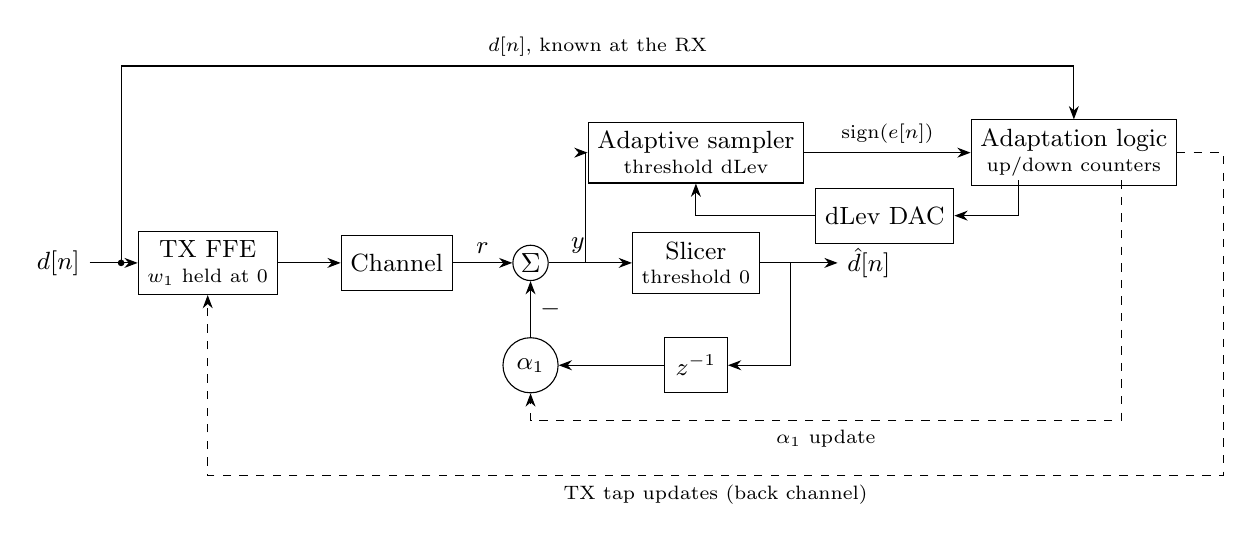
\begin{tikzpicture}[x=1cm, y=1cm]
  \node[blk] (ffe) at (0,0) {TX FFE\\[-2pt]\scriptsize $w_1$ held at 0};
  \node[blk] (ch) at (2.4,0) {Channel};
  \node[draw, circle, inner sep=1pt] (sum) at (4.1,0) {$\Sigma$};
  \node[blk] (slc) at (6.2,0) {Slicer\\[-2pt]\scriptsize threshold 0};
  \node[blk, minimum width=8mm] (z) at (6.2,-1.3) {$z^{-1}$};
  \node[draw, circle, inner sep=0.5pt, minimum size=7mm, font=\small] (al) at (4.1,-1.3) {$\alpha_1$};
  \node[blk] (err) at (6.2,1.4) {Adaptive sampler\\[-2pt]\scriptsize threshold dLev};
  \node[blk] (eng) at (11.0,1.4) {Adaptation logic\\[-2pt]\scriptsize up/down counters};
  \draw[->] (-1.5,0) node[left, font=\small] {$d[n]$} -- (ffe);
  \draw[->] (ffe) -- (ch);
  \draw[->] (ch) -- node[above, font=\small] {$r$} (sum);
  \draw[->] (sum) -- node[above, font=\small, pos=0.35] {$y$} (slc);
  \draw[->] (slc.east) -- (8.0,0) node[right, font=\small] {$\hat d[n]$};
  \draw[->] (7.4,0) |- (z.east);
  \draw[->] (z) -- (al);
  \draw[->] (al) -- node[right, font=\small] {$-$} (sum);
  \draw[->] (4.8,0) |- (err.west);
  \draw[->] (err) -- node[above, font=\scriptsize] {$\mathrm{sign}(e[n])$} (eng);
  \fill (-1.1,0) circle (1.2pt);
  \draw[->] (-1.1,0) |- (11.0,2.5) node[pos=0.75, above, font=\scriptsize] {$d[n]$, known at the RX} -- (eng.north);
  \node[blk] (dac) at (8.6,0.6) {dLev DAC};
  \draw[->] (10.3,1.05) |- (dac.east);
  \draw[->] (dac.west) -| (err.south);
  \draw[->, dashed] (11.6,1.05) -- (11.6,-2.0) -| (al.south) node[pos=0.25, below, font=\scriptsize] {$\alpha_1$ update};
  \draw[->, dashed] (eng.east) -- (12.9,1.4) |- (0,-2.7)
    node[pos=0.75, below, font=\scriptsize] {TX tap updates (back channel)} -- (ffe.south);
\end{tikzpicture}
\caption{TX FFE + 1-tap DFE. The adaptive sampler sees the DFE summer output $y$; the same
$\mathrm{sign}(e)$ updates the TX taps, $\alpha_1$ and dLev (through the dLev DAC).}
\end{figure}

\noindent With $e[n] = \mathrm{dLev} - y[n]$, the DFE tap adds one more counter:
\[
  \alpha_k \leftarrow \alpha_k - \Delta_\alpha\,\mathrm{sign}\Big(\textstyle\sum_n \mathrm{sign}(e[n])\, d[n-k]\Big)
  \qquad(\text{minus: the DFE subtracts}).
\]
\begin{itemize}\itemsep0pt
  \item \textbf{One knob per cursor.} Averaged, $w_j$ drives $p_j$ to 0, $\alpha_k$ tracks $p_k$, and
        dLev tracks $p_0$. A TX post-tap at a cursor the DFE covers is driven by the same
        $p_k-\alpha_k$ as $\alpha_k$, so the split between them would be undetermined: TX post1 is held at 0.
  \item \textbf{All loops together.} The TX equations don't depend on $\alpha$ or dLev; those only
        track cursors the TX sets, so they follow it as it converges.
\end{itemize}

\begin{figure}[H]
\centering
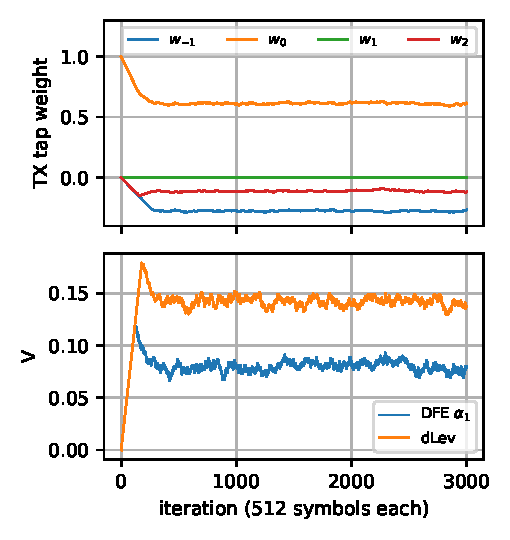
\includegraphics[width=0.42\linewidth]{figures/dfe_convergence.pdf}\hspace{4mm}
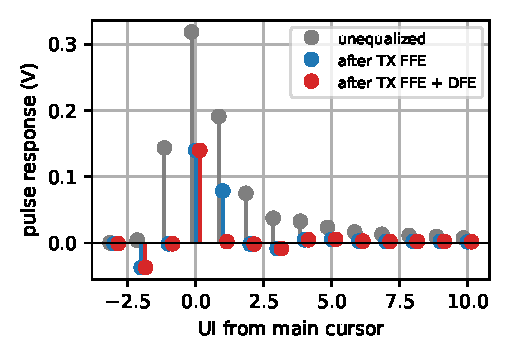
\includegraphics[width=0.42\linewidth]{figures/dfe_pulse.pdf}
\caption{Left: TX post1 ($w_1$) stays at 0 and the main tap settles near 0.6; $\alpha_1$ and dLev
converge with the TX taps. Right: after the TX FFE the first post-cursor remains (blue); the DFE
removes it (red), and the main cursor is about twice the FFE-only one.}
\end{figure}

\begin{figure}[H]
\centering
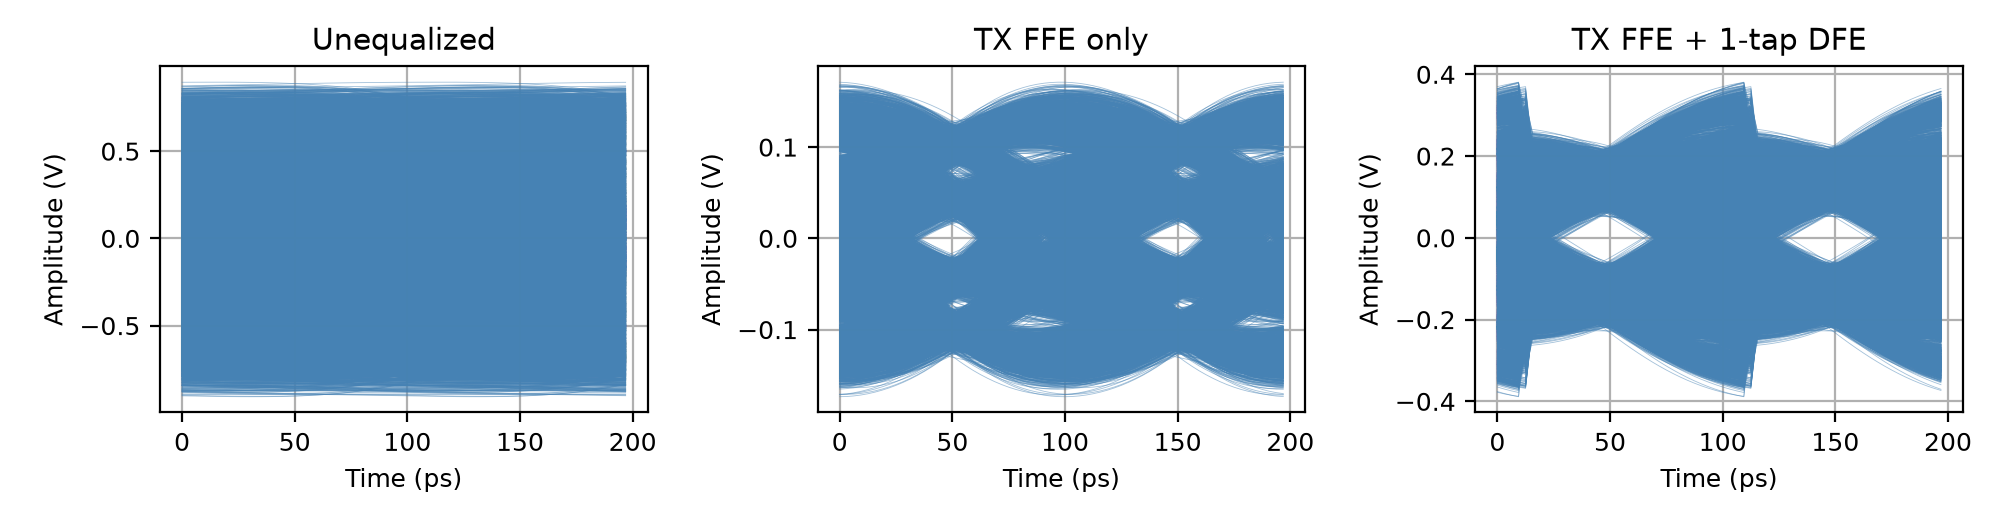
\includegraphics[width=\linewidth]{figures/dfe_eyes.png}
\caption{Waveform-level eyes, 10\,000 random bits. The DFE decides at the pulse-peak instant
from its own past decisions; its feedback is held over the UI centered on that instant
(hence the steps away from the eye center).}
\end{figure}

\begin{table}[H]
\centering\small
\begin{tabular}{lcccc}
\toprule
 & TX taps $[w_{-1}, w_0, w_1, w_2]$ & $\alpha_1$ & main cursor & PDA eye height \\
\midrule
Unequalized & & & 0.319\,V & $-0.622$\,V \\
TX FFE only & $[-0.212, 0.470, -0.256, 0.061]$ & & 0.073\,V & $+0.024$\,V \\
TX FFE + 1-tap DFE & $[-0.278, 0.606, 0, -0.116]$ & 0.077\,V & 0.140\,V & $+0.091$\,V \\
\bottomrule
\end{tabular}
\caption{Adapted settings (mean of the last 500 blocks) and the resulting worst-case eye.}
\end{table}

\noindent\textbf{Takeaways.} The first DFE tap gives most of the gain ($3.8\times$ the PDA eye):
it takes the largest post-cursor without spending swing, so the main tap returns to 0.61.
The TX still has to cancel the pre-cursor (its pre-tap grows to $-0.28$) and now also post2.
In a sweep, more DFE taps saturate near $+0.12$\,V.

\end{document}
